%chapter 5
\chapter{Passenger Transport Operation}
%
\section{Public Transportation}
Public transportation is a generic term used to describe the family of transit services available to urban and rural residents. Thus, it is not a single mode but a variety of traditional and innovative services, which should complement each other to provide system-wide mobility.
%
\subsection{Transit Modes}
The modes included within the realm of public transportation are:
\begin{itemize}
	\item \textbf{Mass transit}, characterized by fixed routes, published schedules, designated networks, and specified stops. Mass-transit vehicles include buses, light rail (trolleys) or rapid transit that either share space in mixed traffic or operate on grade-separated rights of way.
	\item \textbf{Paratransit} is characterized by flexible and personalized service intended to replace conventional fixed-route, fixed-schedule mass-transit lines. Paratransit is available to the public on demand, by subscription, or on a shared-ride basis. Examples include taxi, car rental, dial-a-ride, and specialized services for elderly, medical, and other designated users.
	\item \textbf{Ridesharing} (as the name implies) is characterized by two or more persons traveling together by prearrangement, such as carpool, vanpool, or shared-ride taxi.
\end{itemize}
Buses are the most common transit mode. They operate on streets and have an extensive network of lines. In some cities they have been upgraded by provision of exclusive bus lanes and provision of bus preferential signals.\\\\
Light Rail Transit (LRT) represents the most common mode of semirapid transit. Its articulated electric vehicles operated in short trains on largely separated tracks provide more attractive and permanent services than buses at a much lower investment cost than metro systems require. LRT is presently being developed in many cities around the world that want to make transit services more efficient and largely independent of traffic congestion.\\\\
Metro systems have by far the highest performance - capacity, speed, reliability - of all transit modes. They require very high investment, but in the long run they are essential for efficient functioning and quality of life in large cities.\\\\  
Transit modes are defined by their right-of-way (ROW) category, technology and types of operations. Three ROW categories are:
\begin{itemize}
	\item \textbf{\textit{ROW Category C :}} It represents public streets with general and mixed traffic. Street transit modes include mostly buses, but also trolleybuses and tramways/streetcars. 
	\item \textbf{\textit{ROW Category B}}: It represents transit ways that are partially separated from other traffic. Typically they are street medians with rail tracks, which are longitudinally separated, but
	cross street intersections at grade. Bus lanes physically separated from other traffic also represent ROW category B. This ROW requires a separate strip of land and certain investment for construction.
	\item \textbf{\textit{ROW Category A}}: It is fully separated, physically protected ROW on which only transit vehicles operate. This category includes tunnels, aerial (elevated) structures or fully protected at-grade tracks or roadways. Thus, vertical position of the ROW is not as important as its separation from other traffic, because total independence of TUs allows many physical and operational features that are not possible on ROW categories B and C. Therefore, the modes with ROW category A are guided (rail, exceptionally rubber-tired) systems with trains, electric traction and signal control which offer very high capacity, speed, reliability and safety.
\end{itemize}
%
\subsection{Transit Capacity and Level of Service}
A basic attribute of any transit mode is its carrying capacity, defined as the number of vehicles or persons that pass a given point in a specified time (usually an hour). The numerical value of carrying capacity (usually referred simply as capacity), is dependent on two variables: (1) the number of vehicles that pass a point at a given time and (2) the number of passengers within each vehicle. For example, if for a given lane along a section of highway there are 60 buses that pass by in an hour (or one per minute), and each bus carries 50 seated passengers, then the carrying capacity of this highway lane is 60 buses/ln/hr or $50 \times 60 = 3000$ passengers/ln/hr.\\
\par
Carrying capacity is influenced by (1) the “spacing” in seconds between each
vehicle (called the headway) and (2) the “comfort factor” experienced by passengers (called the level of service). Thus, carrying capacity can be increased in two ways: (1) reduce the headway or (2) increase the number of passengers per vehicle. In the bus capacity example, the headway was 60 seconds and the level of service was that all passengers had a seat. Time spacing between buses could possibly be reduced, but there are limits to lowering headway values dictated by safe distance requirements between vehicles and/or the time spent at transit stops and terminals (called dwell time). Similarly, passenger loading could be increased by allowing standees, but this would decrease the comfort level for passengers. Were the bus equipped with computer tables and a refreshment area (thus offering a higher level of service), fewer passengers could be accommodated resulting in a lower carrying capacity but a higher level of service.\\
\par
Accordingly, when reporting transit capacity, it is important to specify the units
as either vehicles or passengers/hour and the corresponding level of service in terms of passengers/vehicle. Public transit is often compared with the automobile when issues of carrying capacity are involved, as it is commonly believed that transit capacity is superior to auto capacity. The capacity of a single lane of passenger vehicles is approximately 2,000 vehicles/hour which represents a headway of 1.8 seconds. Since most cars have at least five seats, the person capacity of a highway lane could be as great as $ 5 \times 2000 = 10000 $ per/hour. Capacities of this magnitude never have been achieved, since most cars carry only one person with an average car occupancy of about 1.5. Why is this so? Have you ever driven in a car carrying five people? Not a pleasant experience, and a reason why car pooling is not very popular. Given the opportunity, most people choose to drive alone or with just one other person.\\
\par
Travelers usually consider many more factors than simply the in-vehicle level of
service, and they don’t really consider how they can contribute to increasing “carrying capacity.” In fact, if drivers were to optimize the carrying capacity of a highway, they would all drive at 35 miles per hour! Other major considerations in selecting the travel mode include: reliability, punctuality, cost, travel time, and safety. Transit systems that receive “high marks” for the out-of-vehicle level-of-service factors are typically the ones that use exclusive lanes or tracks with no interference from other vehicles or pedestrians and have adequate capacity at station stops and terminals. Thus, rapid transit services (whether bus or fixed guideway), are the superior mode but are more costly to build and maintain and require high volumes of demand to be feasible.
%
\subsection{The Role and Future of Public Transportation}
Public transportation is an important element of the total transportation services provided within large and small metropolitan areas. A major advantage of public transportation is that it can provide high-capacity, energy-efficient movement in densely traveled corridors. It also serves medium- and low-density areas by offering an option for auto owners who do not wish to drive and an essential service to those without access to automobiles, such as school children, senior citizens, single-auto families, and others who may be economically or physically disadvantaged.\\
\par
For most of this century, public transportation was provided by the private sector.
However, increases in auto ownership, shifts in living patterns to low-density suburbs, and the relocation of industry and commerce away from the central city, along with changes in lifestyle (which have been occurring since the end of World War II) have resulted in a steady decline in transit ridership. Since the early 1960s, most transit services have been provided by the public sector. Income from fares no longer represent the principal source of revenue, and over a 25- to 30-year period, the proportion of funds for transit provided by federal, state, and local governments has increased steadily. While it generally is believed that highways and motor transport will play a dominant role in providing personal transportation in the beginning decades of the twenty-first century, there are many unforeseen changes that could alter the balance between public and private transportation. Some could contribute to a decline in transit ridership while others might cause transit to become stronger, and for the remainder, there would be little or no effect. The potential changes that could influence transit usage are categorized here from the book Urban Mass Transportation Planning.
%
\subsubsection{Factors Bad for Transit}
\begin{itemize}
	\item Growth of suburbs
	\item Industry and employment moving from the central city
	\item Increased suburb-to-suburb commuting
	\item Growth in private vehicle ownership
	\item Increased diversity in vehicle types such as SUVs, pickup trucks, and RVs
	\item High labor costs
\end{itemize}
%
\subsubsection{Factors Good for Transit}
\begin{itemize}
	\item Emphasis by the government on air quality
	\item Higher prices of gasoline
	\item Depletion of energy resources
	\item Trends toward higher-density living
	\item Legislation to encourage “livable cities” and “smart growth”
	\item Increased number of people who cannot or choose not to drive 
\end{itemize}
%
\section{Bus Transit System}
Buses represent the most widely used transit technology. Virtually every city in the world that has transit service operates buses. Large cities with rail transit also operate extensive bus networks, usually on lines with lower passenger volumes or as feeders to rail lines.\\\\
Bus service is easy to introduce or modify: basic service requires only purchase of vehicles, garage and maintenance facilities, and organization of service. Stops along the lines can be simple. Therefore, buses represent the most economical transit mode for lightly traveled lines. This flexibility of bus routes is an advantage for any necessary changes, but it is a disadvantage for major bus lines: they lack permanence, efficiency in
carrying heavy passenger volumes, and image of permanent, physically fixed routes desired by passengers.\\\\
Compared to paratransit modes, bus transit is very labor-efficient: one driver operates a vehicle with capacity of 50-150 spaces. Compared to rail transit, buses are labor-intensive and have no economy of scale: on heavily traveled lines, for every additional 40-120 passengers, one bus and one driver must be added to the service.
\subsection{Bus Vehicles}
There is a range of bus vehicles by their size/capacity and body type. Some of the major types are discussed below:
\begin{description}
	\item [Minibus] is a 6-8 meters long vehicle, which has a capacity of 15-40 seats and standing spaces. It is used for lightly traveled lines, short shuttle lines, services in residential neighborhoods, etc.
	\item [Regular Bus]
 is 10-12 m long, 2.50 m wide. It has 30-50 seats and 60-20 standing spaces (minimum number of seats corresponds to the maximum number of standing spaces)
	\item [Articulated Bus] is a vehicle with the main body on two axles and an articulated section with the third axle. With their greater capacity, articulated buses are suited for heavily traveled lines. In few cities, with very heavy ridership, double-articulated buses with three body sections and four axles are used.
	\item [Double-decker Buses] have two decks, the upper being for seated passengers only. Like articulated buses, double-deckers have a greater capacity than regular buses, but take less street space. They involve passengers climbing stairs, which is inconvenient. Riding on the upper deck, however, offers nice views for passengers. They are used extensively in the cities of the United Kingdom and many British Commonwealth countries, as well as in Berlin and a few other cities.
	\item [Low Floor Buses], perfected during the 1990s, have become standard in several industrialized countries. These buses have floors 35-40 cm above ground, so that entry from a curb is nearly flat, or a plate is provided for wheelchairs. Low-floor buses offer considerably greater comfort for passengers and speed up their boarding-alighting. Mechanical equipment on these buses is stored mostly on the roof, while the motor is in a compartment in the rear, where the floor is ramped up.
\end{description}
In selecting buses for a specific service, expected passenger volume is critical for vehicle design. Maneuverability and riding comfort are also considered. Thus, for lightly traveled bus lines in suburban areas with many narrow residential streets, or on hilly terrain, a minibus may be best suited because it is least expensive per vehicle-km, its small capacity
is adequate and it can negotiate such alignments better than large buses. On the other hand, heavy passenger loads make regular or high-capacity buses more economical and superior in offering the required capacity. Average trip lengths influence the number and width of doors, as well as seating arrangement.\\\\
Relatively short trips and intensive exchange of passengers at stops requires two double channel doors on regular, 3 - 4 double channel doors on articulated buses, and single rows
of seats on each side. For lines with moderate passenger loads and longer trips, 2+1 or 2+2 seating may be used. In the latter case, standing should be expected only in exceptional cases. In all cases access for passengers in wheelchairs is legally required to be provided by lifts, “kneeling bus” which can be lowered in the front, or by low-floor bus design.\\\\
\subsection{Bus Travelways}
The vast majority of buses operate on regular streets, ROW category C. Being in mixed traffic, their speed and reliability of service depend on traffic conditions. Their average speed is lower than the average speed of cars because they stop to pick up and drop off passengers. Buses are therefore not very competitive with car travel in the same corridor with respect to speed and reliability. Their advantages are much lower cost and convenience of not having to drive and park.\\\\
To make buses more efficient and attractive to passengers, bus preferential measures can be introduced. These include the following:
\begin{itemize}
	\item \textbf{\textit{Preferential signals}}: buses in a separate approach lane at intersections get the green signal before other lanes, so that they can proceed through the intersection ahead of other traffic.
	\item \textbf{\textit{Alternating stop locations}} at near- and far-side of intersections (before or after cross street) so that buses clearing one intersection on green signal use the green at the following intersection before they make the next stop. Also, spacing between bus stops should typically be about 250-400 m.
	\item \textbf{\textit{Exclusive bus lanes}}, which may be curb lanes or lanes in the median - ROW category B. This is the most significant improvement measure because it makes buses independent of traffic conditions on the same street.
	\item \textbf{\textit{Buses on high-occupancy vehicle (HOV) lanes or roadways}} are used when bus lines with frequent service follow freeway alignment for a rather long distance. HOV facilities usually have traffic control that prevents congestion, but they do not provide the image of an exclusive, independent transit facility.
	\item \textbf{\textit{Busway}} - special roadways reserved for buses only (ROW category B or A). Since busways require very high investment costs, they are used for some sections of lines. If ROW category A is required for a large section of line, it is usually better to introduce a rail system, so that the investment in high quality ROW is better used for electrically powered trains, rather than single bus vehicles
\end{itemize}

%
\section{Number of Passengers Versus Number of Served Vehicles}
Traffic engineers try by various techniques and measures to enable as many vehicles as possible to pass,
during a specific period of time, through a traffic intersection or through a road section. In other words, traffic experts try to maximize the number ofvehicles that are served during a certain period of time. On the other hand, when it comes to public transit, we are trying to maximize the number of transported passengers. The number of passengers that can be served during the observed time interval represents transit line capacity. Similarly, the number of vehicles that can be served during the observed time interval represents the vehicle line capacity.
\subsection{A Hypothetical Case Study}
Let us assume that the freeway lane can serve 2200 vehicles per hour (the freeway lane capacity equals 2200 vehicles per hour). The upper part of the figure shows the situation when only private cars used freeway lane. The lower part of the figure refers to the situation when some buses also participate in freeway lane traffic. We assume that average number of passengers in bus and private car (average occupancies) are, respectively, equal to 50 and 1.4. We also assume that instead on any two private cars we can allow one bus to participate in freeway lane traffic.\\
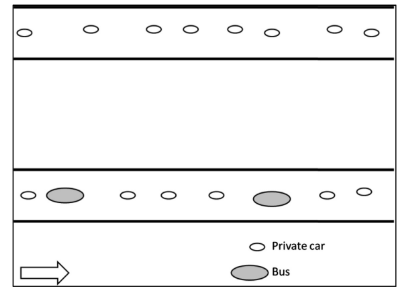
\includegraphics[scale=0.8]{gfx/fig15.png}\\
We denote by C, B, and P, respectively, the total number of cars, total number of buses, and total number of transported passengers. Ifwe allow, for example, 50 buses to enter the freeway lane, we need to reduce the total number of private cars for $ 50 \times 2 = 100$ private cars.In this case, the total number of transported passengers P by private cars and buses equals:\\\\
$ P = C \times 1.4 + B \times 50 = 2100 \times 1.4 + 50 \times 50 = 5440$ Passengers\\\\
The table and the graph below show increase in the total number of transported passengers with the increase of the number of buses engaged.\\
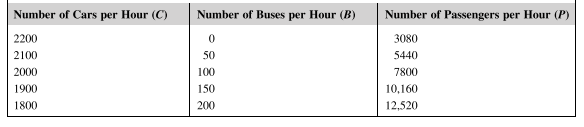
\includegraphics[scale=0.8]{gfx/fig16.png}\\
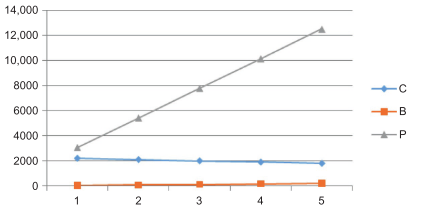
\includegraphics[scale=0.8]{gfx/fig17.png}\\
%
The graph above illustrates the effects that public transit can achieve. With a very small percentage share of public transport vehicles in the total number of vehicles, it is possible to increase dramatically the total number of passengers carried. To achieve such effects in reality, it is necessary constantly to increase the public transit attractiveness.
%
\section{Passenger Flows in Public Transportation}
Passenger flows vary considerably in public transportation. During the working day, in most cities in the world, the daily numbers of passengers on most transit lines are relatively uniform. This is due to the fact that many passengers, each working day, use the same transportation mode and the same route when going to work. During a weekend the number of passengers in public transit is significantly smaller. The figure below shows daily variations in passenger volume.\\
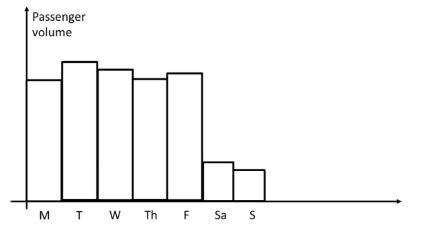
\includegraphics[scale=0.7]{gfx/fig18.png}\\
The fig below shows hourly variations in passenger volume. The variations shown in figure are typical for many cities in the world. There are morning and evening peaks when people go, and when people come back from work.The differences in hourly passenger volumes could be very high by hours of a day.\\
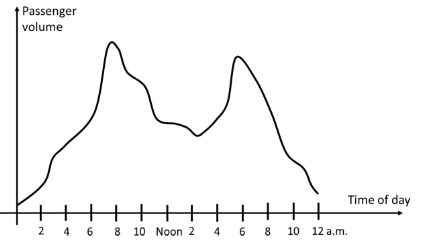
\includegraphics[scale=0.7]{gfx/fig19.png}\\
Hourly variations in passenger volume have, as a consequence, different number of vehicle departures from the terminals during certain time intervals as shown in the figure below. In this way, hourly variations in passenger volume require the engagement of different number of vehicles during certain time periods. The number of engaged vehicles is much higher during the rush-hours. Outside the peak periods the transit operator has a surplus of vehicles and drivers. The transit operator, therefore, meets with a range of organizational problems that have to be solved (“empty” vehicle trips to garage and from garage, drivers working hours divided in two shifts, vehicle maintenance planning, etc.).\\
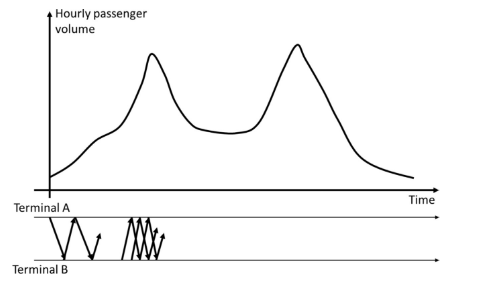
\includegraphics{gfx/fig20.png}\\
%
\section{Passenger Flows Along a Transit Line}
Headway in public transportation operations represents the time interval between vehicles past a specific point as shown in the fig below. Headways are expressed in minutes. It is essential to study passenger flow along the transit line, in order to determine the appropriate transit line headway.\\
\par
Let us assume that we have data on the number of boarding passengers and number of alighting passengers on individual line stops and terminals (end stations on a transit line) as shown in the table below. The transit line has 5 stations. The terminals are denoted respectively by A and B.\\
\par
The last column of the table shows the numbers of passengers in the vehicle, after departing from bus stops. Thus, for example, after leaving the station 2, there are 21 passengers in the vehicle that travels along line section between stop 3 and stop 4. The number of boarding passengers, number of alighting passengers and the number of passengers in the vehicle for any line section are shown in the figure below.\\
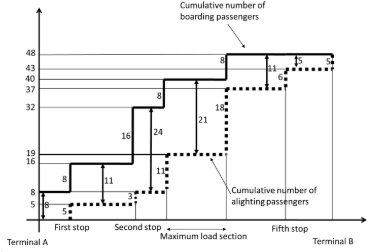
\includegraphics{gfx/fig21.png}\\
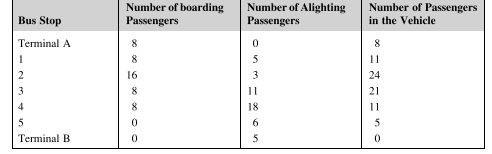
\includegraphics{gfx/fig23.png}\\
%
The numbers of passengers on certain line sections respectively equal 8, 11, 24, 21, 11, and 5. The maximum passenger volume equals max ${8, 11, 24, 21, 11, 5} = 24$ and corresponds to the section between stop 2 and stop 3. We call section between stop 2 and stop 3 the maximum load section (MLS).\\\\
The data shown in the table and figure above are related to one vehicle trip. In real-life applications, 1 h is the basic time unit that is used when describing cumulative number of alighting and boarding passengers, as well as the maximum passenger volume on MLS. In other words, the maximum passenger volume is expressed in passengers per hour. The passenger volume profile is calculated for both directions of the transit line.\\\\
In the figure shown below, the line length is denoted by L. This length represents the one-way distance between the line terminals along the line alignment. The line length is measured in miles or kilometers. We denote by qi passenger volume on the $ i^th $ section. The length of the $ i^th $ transit section is denoted by li. The MLS in one direction is usually different from the MLS in another direction. The maximum passenger volumes in both directions should be taken into account when determining the number of vehicles to be engaged on the transit line.\\
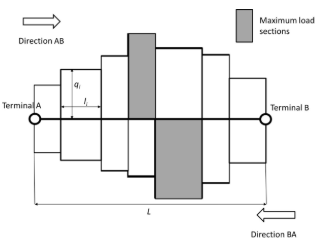
\includegraphics{gfx/fig22.png}
%
\section{Service Frequency and Headways}
One of the most important problems encountered by public transit operators is how to match transportation supply and passenger demand on individual transit line. The matching problem is far more complex over the entire route network than on individual routes. Service frequencies and vehicle departure times on transit lines in the network reflect the manner in which transportation supply and passenger demand are matched. Service frequencies and vehicle departure times depend on passenger volume profile and on the number and type of vehicles in the fleet. The number of passengers that decide in the end to use public transit on a particular transit line depends, to the highest degree, on service frequency and vehicle departure times. For example, if service frequency is low or if vehicle departure times during the day are not convenient, a number of potential passengers will instead choose other modes of transportation.\\
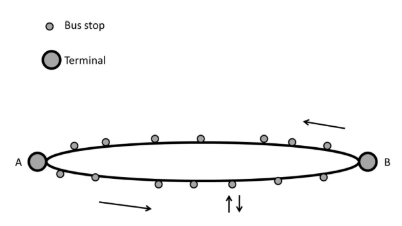
\includegraphics{gfx/fig24.png}\\
Let us note the bus line shown in the figure above. Vehicles move from Terminal A to Terminal B. On the way to the Terminal B, vehicles stop at pre-defined bus-stops, where passengers enter and exit the vehicle. On arrival at the Terminal B, the driver rests for a while, and then the vehicle travels to Terminal A. On the way to Terminal A, car stops at bus-stops where passengers enter and exit the vehicle.\\\\
We denote by T turnaround time. This time is the time that elapses from the moment when vehicle leaves Terminal A to the moment when vehicle returns to Terminal A. Let us assume that we have on our disposal N vehicles that we can assign to the bus line. The service frequency represents the number of vehicles per time unit past a specific point in the same direction. The frequency equals:
\begin{equation}
	f = \frac{N}{T}
\end{equation}
The frequency is expressed in the number of vehicle per hour. Headway h in public transportation operations represents the time interval between vehicles past a specific point. Headways are expressed in minutes. Since the frequency represents the number of vehicles per time unit past a specific point in the same direction, we conclude that the frequency is the inverse of the headway, ie:
\begin{equation}
	h = \frac{1}{f}
\end{equation}
When calculating and rounding headways, it is desirable to obtain a so called clock headway. Clock headways have a feature that enables the generation of timetable that is repeated every hour, starting on the hour. Thus, for example, in the case when the headway is equal to 15 min, it is possible to have the vehicle departures from the terminal in 8:00, 8:15, 8:30, 8:45, 9:00, 9:15, 9:30, 9:45, 10:00, etc.
%
\subsection{The Maximum Service Frequency}
The maximum service frequency is defined by the maximum number of transit vehicles passing through a given point of a line/route i in one direction during a given period of time (usually 1 h) under prevailing operating conditions. This can be estimated as follows:
\begin{equation}
	\label{maxServiceFreq}
	f_{max/i}(\tau) = \frac{\tau}{h_{min/i}}
\end{equation}
Where,\\
\hspace*{10mm} $\tau$ is the given period of time\\
\hspace*{10mm} $h_{min/i}$ is the minimum headway, ie, the time interval between the successive transit vehicles passing through a given point of a line/route i in the same direction (min).\\\\
The minimum headway $ h_{min/i} $ in Eq. \ref{maxServiceFreq} can be determined according to different criteria, but in many cases the prevailing factors are characteristics of the system such as technology and way of operations along the line and at the stations. These factors influence the minimum headway for a given line line/ route and for the stops/stations along it. Most frequently the stop/station headway is as much greater than that of the line(s)/route(s). In addition, the headway $ h_{s/i} $ at the stop/station on a given line/route i, should be greater than the vehicle stop time $ t_{s/i} $ at that stop/station. Consequently, the “ultimate” capacity of this stop/station will be:
\begin{equation}
	C_{ss/i}(\tau) = \frac{\tau}{max[h_{s/i}, t_{s/i}]}
\end{equation}
In addition, the following must be satisfied for all stops/stations on the line/route i:
\begin{equation}
	f_{max/i}(\tau) \leq C_{ss/i}
\end{equation}
In other words, the maximum number of transit vehicles passing through a given stops/stations cannot exceed the “ultimate” capacity of any of these stops/stations.
%
\subsection{Passenger Waiting Time}
Passengers’ walk to a stop and passenger waiting time are the basic attributes of the public transit level of service. Walk to stop in the range of 400–800 m is considered acceptable for public transit users.\\\\
In order to estimate the average passenger waiting time, let us first consider the situation when the bus arrives at the bus stop regularly, according to the published timetable. We also assume that all passengers at the bus stop can enter the vehicle, and that the passengers appear at the bus stop in random moments of time. It has been shown that, in this case, the average waiting time per passenger at the station w is equal to the one half of the vehicle headway $ h $, ie:
\begin{equation}
	w = \frac{h}{2}
\end{equation}
The average waiting time per passenger could be longer in the case of irregular bus arrivals. In the case of irregular bus arrivals, vehicle headway is not any more deterministic quantity. In this case, the vehicle headway is a random variable. If the planned headway equals, 10 min, in the case of irregular arrivals headway values could be, for example, 8, 9, 12, 15,…. minutes. It has been shown, that in the case of irregular vehicle arrivals at the stop, the average passenger waiting time equals:
\begin{equation}
	E(W) = \frac{E(H)}{2} + \frac{var(H)}{2 \times E(H)}
\end{equation}
Where, $ E(H) $ is the expected value of the random variable H; and $ var(H) $ is the variance of the random variable $ H $ (variance represents the square of standard deviation).
%
\subsection{Headway Determination by "Square Root Formula" }
Transit operator cost and passenger cost depend on chosen headway. Passenger cost, in the case when vehicles arrive regularly, has linear increase with headway. The greater the headway, the greater the passenger waiting time and passenger cost. On the other hand, greater headway means for transit operator smaller number of departures and lower costs.
\begin{description}
	\item $ Z $ is the total cost per hour;
	\item $ c $ is the transit operator cost per bus hour;
	\item $\nu$ is the value of passenger waiting time per hour;
	\item $ r $ is the total number of passengers on line per hour (ridership per hour);
	\item $ N $ is the number of vehicles assigned to the bus line; and
	\item $ h $ is the headway.
\end{description}
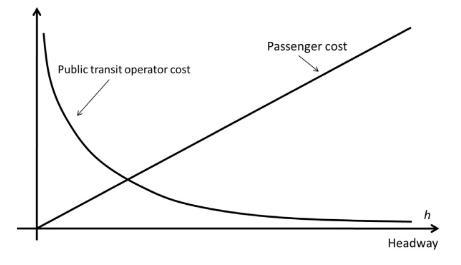
\includegraphics{gfx/fig25.png}\\
The transit operator cost per hour is equal to $N \times c$. We assume regular vehicle arrivals. In this case, the average waiting time per passenger at the station $ w $ is equal to the one half of the vehicle headway $ h $, ie:
\begin{equation}
	w = \frac{h}{2}
\end{equation}
The waiting cost of all passengers is equal to the $ \nu \times r \times \frac{h}{2} $. The total cost is:
\begin{equation}
	Z = N \times c + \nu \times r \times \frac{h}{2}
\end{equation}
Since, $ N = \frac{T}{h}$, we can write,
\begin{equation}
	Z = \frac{T}{h} \times c + \nu \times r \times \frac{h}{2}
\end{equation}
The optimal headway is found by setting the derivative of $ Z $ with respect to $ h $ equal to zero:
\begin{equation}
	\frac{dZ}{dh} = -c \times \frac{T}{h^2} + \frac{\nu \times r}{2} = 0
\end{equation}
Therefore the Optimum Headway,
\begin{equation}
	\label{headwaySqrt}
	h = \sqrt{\frac{2 \times c \times T}{\nu \times r}}
\end{equation}
Eq. \ref{headwaySqrt} represents the “square root formula” for optimizing headway and service frequency. Minimal headway values in real-life are usually between 2 and 3 min. Maximal headways values are between 15 and 30 min. Outside of peak periods, on some transit lines, maximum headway values reach 60 min.\\\\
The service frequency $ f $ is the inverse of the headway, ie:
\begin{equation}
	f = \frac{1}{h} = \sqrt{\frac{\nu \times r}{2 \times c \times T}}
\end{equation}
Service frequency dependence of the total number of passengers on line per hour is shown in the figure below.\\
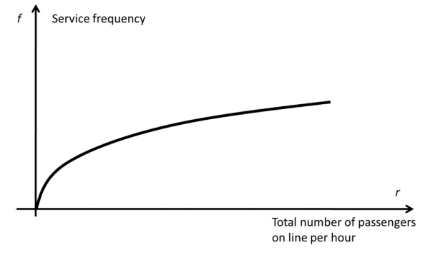
\includegraphics{gfx/fig26.png}\\\\
\textit{Numerical Example:}\\
Let us assume the following line parameters: $ c $ = 120\$ per hour, $ \nu $ = 10\$ per passenger hour, $ r $ = 1200 passengers per hour, and $ T $ = 1.5 hr. Calculate the optimal headway.\\
\textit{Solution:}\\\\
$ 	h = \sqrt{\frac{2 \times c \times T}{\nu \times r}} = \sqrt{\frac{2 \times 120 \times 1.5}{10 \times 1200}} = 0.173 hr$\\\\
$ \therefore h \approx 10 min$
\subsection{Headway Determination by Maximum Load Method}
When determining headways, transit operators try to provide enough space (especially during peak hours) to meet passenger demand. Majority of transit operators also define maximum headways on transit lines. For example, operator could define that maximum headway on a specific route, is equal to 30 min. Maximum headways guarantee a minimum service frequency offered to the passengers. The prescribed maximum headway is usually called \textit{policy headway} and denoted by $ h_p $.\\\\
The Maximum load method (that can have few variations) is based on counting passengers on the transit stop that is at the beginning of the MLS. Depending on the time of a day, the location of the MLS could change. For example, the transit stop, that is at the beginning of the MLS, could be Stop \#5 between 10:00 am and 11:00 am, while Stop \#7 could be at the beginning of the MLS between 5:00 pm and 6:00 pm Frequently, passenger counting is performed at the bus stop that has the highest daily passenger volume. The location of this transit stop is usually well known to the transit operator. The counting interval (whole day, between 7:00 am and 10:00 am, between 4:00 pm and 7:00 pm, etc.) is different for different transit operators and different cities.\\\\
We denote by $ P_{max} $ the average value of the maximum daily passenger volume. For example, transit operator monitored during seven days period the daily number of passengers that departed from the station \# 6. The following 7 values were recorded: 1262, 1348, 1439, 1285, 1290, 1391, and 1287. The $ P_{max} $, in this case is equal to:
$$ P_{max} = \frac{1262 + 1348 + 1439 + 1285 + 1290 + 1391 + 1287}{7} = 1329 $$
%
The service frequency, $ f $, that should be offered in order to satisfy maximum passenger volume and desired vehicle occupancy is equal to:
\begin{equation}
	f = \frac{P_{max}}{\alpha \times C_{car}}
\end{equation}
Where, $ C_{car} $ is maximum number of passengers per car; and $ 0 \leq \alpha \leq 1$ is load factor.\\\\
The Load factor $ \alpha $ is related to the concept of desired vehicle occupancy. The product $ \alpha \times C_{car} $ defines the desired vehicle occupancy during the observed time period.\\\\
The corresponding headway is equal to:
\begin{equation}
	h = \frac{1}{f} = \frac{\alpha \times C_{car}}{P_{max}}
\end{equation}
%
\section{Time Table}
The transit line timetable is generated at one point (usually terminal). In the next step, by using information about average travel times between transit stops, timetable is generated for all transit stops. The transit operator’s timetable contains information about vehicle departure times at all transit stops.\\\\
ansit operator’s timetable contains information about vehicle departure times at all transit stops. The basic input data for the timetable construction represent service frequency values in certain intervals of time during the day. Timetable can easily be generated in the following way. Let the abscissa represents time. Based on the known values of service frequency in certain intervals of time, we draw a cumulative frequency.\\
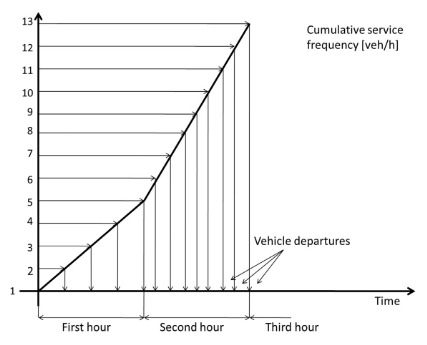
\includegraphics{gfx/fig27.png}\\
The cumulative frequency shown in the figure above is related to the case when service frequency within first hour is equal to 4, and service frequency within second hour is equal to 8. Let us first vehicle departure happen at the beginning of the first hour. We can go horizontally for every vehicle departure, until intersecting the cumulative curve. From the point of intersection we go vertically. The intersection of this vertical line and abscissa represents vehicle departure time. In this way, we generate timetable at specific point. In this way, we generate constant headways during specific time intervals.\\\\
Because of demand variability, constant headways frequently do not generate equal number of passengers at every vehicle departure. In order to achieve even-load at every vehicle departure, we draw cumulative loads on the transit stop that is at the beginning of the MLS.\\
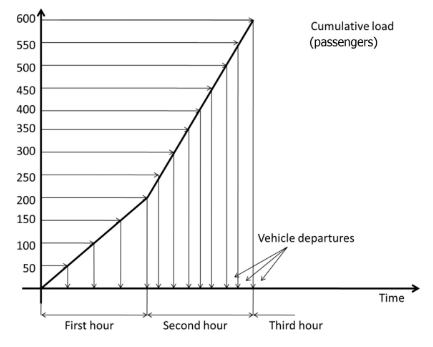
\includegraphics{gfx/fig28.png}\\
Unequal number of passengers at specific vehicle departures can cause overcrowding in some vehicles, long boarding time at some transit stops, “bunching” of vehicles, and a decrease in the level of service offered to the passengers. On the other hand, equal load is related to unequal headways which could be inconvenient for passengers.\\\\
Trips between nodes in public transit networks may be made with or with no making transfers.
Transfers generally cause inconvenience to passengers. Given that inadequately coordinated transfers can increase waiting times considerably, it is particularly important (when constructing timetables) to synchronize schedules cautiously in cases of larger headways. Unsuccessfully coordinated transfers can also reduce the number of passengers using public transit as a result of switching to competitor modes. When designing synchronized schedules, it is essential to try to minimize the total waiting times of all passengers at transfer nodes in a transit network.
%
\section{Transit Line Capacity}
The transit line is the basic element of public transit system. The transit route lengths in one direction are usually between 40 and 90 min, while stop spacing in urban areas are in the range from 120 to 400 m. It is desirable that transit route intersects few other transit routes. In this way, transfer points are generated that enable passengers to create various itineraries when making a trip. The waiting time at transfer points, which is less than 8 min, is considered as an acceptable waiting time. The transit line operating hours by weekdays are usually between 5:00 am and midnight. The spacing between transit lines, in the majority of cities, is in the range of 700–1000 m.\\\\
We denote by $ C_{car} $ the maximum number of passengers per car. Bus capacity represents the sum of number of seated passengers and legal standees. Public transit agencies and operators usually assume six passengers per square meter, as legal standees. In some countries, this figure could be higher.
\\\\
The line/route (offered) “ultimate” capacity $ C_{car}(\tau) $ is expressed by the maximum number of spaces, which can be transported in one direction during a given period of time $\tau$ (usually 1 hr) under prevailing operating conditions. In other words, the “ultimate” capacity of a public transportation lines represents the product of the maximum frequency of the service $ f_{max}(\tau) $ and the maximum number of passengers in the transit vehicle.
$$ C_{car}(\tau) = f_{max/i}(\tau) \times N_{car} \times C_{car} $$
%
The practical capacity $ C_{line} $ of a public transit line represents the product of the offered service frequency $ f $ and the maximum number of passengers in the transit vehicle.
\begin{equation}
	C_{line} = f \times N_{car} \times C_{car}
\end{equation}
Where, $ N_{car} $ is the number of cars/vehicles, and $ C_{car} $ s the maximum number of passengers per car.
\\\\
The number of vehicles $ N_{car} $ per service frequency $ f $ can be variable. In the case of bus operations, $ N_{car} = 1 $ , and the capacity of a public transportation line $ C_{line} $ equals:
\begin{equation}
	C_{line} = f \times C_{car} (spaces/hr)
\end{equation}
The turnaround time equals:
\begin{equation}
	T = \frac{2 \times L}{u}
\end{equation}
Where, $L$ is the distance between Terminals A and B (for simplicity we assume that distance from A to B is equal to the distance from B to A); and $u$ is the average vehicle speed.\\\\
Then,
\begin{gather}
	C_{line} = \frac{N}{T} \times C_{car}\\
	C_{line} = \frac{N}{\frac{2 \times L}{u}} \times C_{car}\\
	\therefore C_{line} = \frac{N \times u \times C_{car}}{2 \times L}
\end{gather}
As we can see, the line capacity $ C_{line} $ depends on the number of engaged vehicles $ N $, the average speed $u$, vehicle capacity $C_{car}$, and length of the line $L$. By changing some of these quantities, it is possible to change line capacity.\\\\
\textit{Numerical Example:}\\
The public transit line length equals 10 km in one direction. The average bus speed on a city heavy traffic equals 20 km/h. The total of 12 buses is assigned to the line. The capacity of every vehicle equals 50. Calculate the line capacity, frequency, and headway.\\
\textit{Solution:}\\\\
The Line Capacity,\\\\
$ C_{line} = \frac{N \times u \times C_{car}}{2 \times L}$\\\\
$ C_{line} = \frac{12 \times 20 \times 50}{2 \times 10}$\\\\
$ \therefore C_{line} = 600 (spaces/hr)$\\\\
Then,\\\\
$ T = \frac{2 \times L}{u} = \frac{2 \times 10}{20} = 1 hr$\\\\
We have,\\\\
$ f = \frac{N}{T} = \frac{12}{1}$\\\\
$ \therefore f = 12 vehicles/hr$\\\\
Also,
$ h = \frac{1}{f} = \frac{1}{12} = \frac{1}{\frac{12}{60}}$\\\\
$ \therefore h = 5 minutes$
%
\subsection{Transit Line Capacity Utilization}
The transit line capacity represents the number of spaces offered to passengers that pass a specific point in one direction during 1 h. Transit operator offers specific number of spaces to the passengers during specific period of time. It could happen that the offered capacity is insufficient in certain situations. On the other hand, is it possible that the offered capacity is underutilized. Therefore, there is a need to measure the utilization of the offered capacity. The figure below shows transit line capacity and passenger volume profile on the transit line between terminal A and terminal B.\\\\
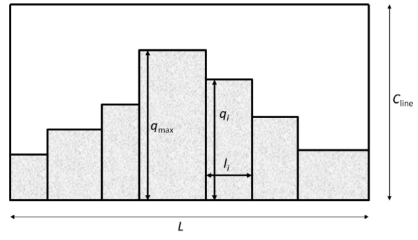
\includegraphics{gfx/fig29.png}\\
The transportation work $ w_i $, made by the transit operator when carrying $ q_i $ passengers along the section that has length equal to $ l_i $, equals:
\begin{equation}
	w_i = q_i \times l_i
\end{equation}
Transit operator offers to the passengers the capacity that is equal to $ C_{line} $. The transportation work that is possible to make is equal to the area of a rectangle with sides $ L $ and $ C_{line} $. The realized transportation work is equal to the sum of the areas of shaded rectangles. The average transit line capacity utilization $\alpha$ is given by:
\begin{equation}
	\alpha = \frac{\sum_{i = 1}^{n} q_i \times l_i}{C_{line} \times L}
\end{equation}
Where $n$ is the number of line sections.
\\\\
\textit{Numerical Example:}
The public transit line length equals 5 km in one direction. The average bus speed on a city heavy traffic equals 20 km/h. The total of 10 buses is assigned to the line. The capacity of every vehicle equals 50. The passenger volume profile of the line is given in the figure below.\\
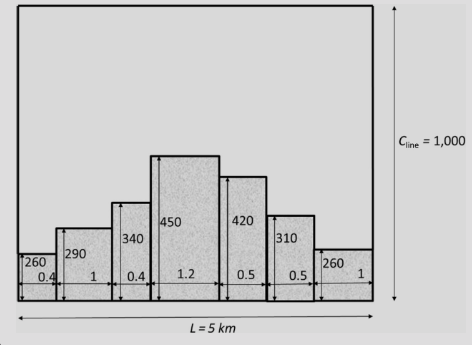
\includegraphics{gfx/fig30.png}\\
Calculate the turnaround time, service frequency, headway, line capacity, and the average transit line capacity utilization $\alpha$.\\\\
\textit{Solution:}\\\\
Turnaround time,\\\\
$ T = \frac{2 \times L}{u} = \frac{2 \times 5}{20} = 0.5 hr$\\\\
$ \therefore T = 30 minutes$\\\\
Then, service frequency:\\\\
$ \therefore f = \frac{N}{T} = \frac{10}{0.5} = 20 vehicles/hr$\\\\
Also, headway:\\\\
$ \therefore h = \frac{1}{f} = \frac{1}{20} = \frac{1}{\frac{20}{60}} = 3 minutes$\\\\
Now, Line Capacity,\\\\
$ \therefore C_{line} = \frac{N \times u \times C_{car}}{2 \times L} = \frac{10 \times 20 \times 50}{2 \times 5} = 1000 spaces/hr$\\\\
Also, the average transit line capacity utilization:\\\\
$ \alpha = \frac{\sum_{i = 1}^{n} q_i \times l_i}{C_{line} \times L} $\\\\
$ \alpha = \frac{260 \times 0.4 + 290 \times 1 + 340 \times 0.4 + 450 \times 1.2 + 420 \times 0.5 + 310 \times 0.5 + 260 \times 1}{1000 \times 5} $\\\\
$ \therefore \alpha = 0.339$
%
\section{Route Development}
A transit system typically consists of many routes on each of which different number of transit units ( for example, buses, trams, street, cars, and the like) ply. A route is a path that a transit unit follows during its journey from the origin terminus to the destination and back. A route is a path that a transit unit follows during its journey from the origin terminus to the destination terminus and back. Along the route there can be many stops at which the transit units halt to let passengers alight and board. The subject of this section is to discuss what constitutes a good set of routes and how we can determine such a set. The next section how we can determine the location of stops on a route.
\subsection{Properties of a Good Route Set}
A transit system's aim or for that matter any public transportation system's aim is to provide transport to a large portion of the population efficiently. In order to achieve this goal, the following properties of a route set are desirable.
\begin{description}
	\item [Ridership:] The percentage of the potential transit users who are served by the designed route set should be as high as possible. Given a route set and a statement of the origins and destinations of the potential transit users, we can determine the above quantity easily. An example is shown later to illustrate how this can be done.
	\item [Riding Time:] The time spent by any passenger on the transit unit should not be more than the time the passenger would have to spend going from his/her origin to his/her destination directly.
	\item [Transfer:] Often in a transit network, we may have to change routes at some intermediate stops to go from the origin to the destination. This changing of routes is referred to as a transfer. The route set should be designed such that passengers are not required to make too many transfers while transfers while travelling from their origins to their destinations.
\end{description}
%
\section{Stop Location and Stopping Policy}
In this section, some issues related to then number of stops (and their locations) to be provided on a route and the stopping policy to be followed by the transit units plying on a route are discussed. The first subsection is on stopping policy and the next on stop locations.
\subsection{Stopping Policy}
Stopping policy relates to the policy followed by the transit system as regards to stopping on the route. There are different stopping policies of which any one may be used by a transit system. These are: (i) All stop, (ii) On-call stop, and (iii) Demand stop.\\\\
In the all stop case, the transit stops at all the stops at all the stops on the route irrespective of whether there is any demand for that stop. For a given transit unit, the demand for a stop exists if someone wants to board the transit unit from the stop or someone on the transit unit wants to alight at that stop. In the on-call stop case, the transit unit stops at a stop if and only if there is a demand for that stop. In the demand stop case, the transit unit stops anywhere along the route where it needs to stop to pick up or drop off passengers. In this case, although the route is fixed, the stop locations are not fixed or alternatively all points on the route are viable stop locations (although the transit unit does not stop at most of them).\\\\
In order to decide which is the best policy for a transit system (or a route in the transit system) a simple analysis, based on the expected number of places at which a transit unit a given route may have to stop, is done. The analysis procedure is shown below.\\\\
Assume that the transit units are operating on a route with $ n $ stops (i.e. stop locations). Note that n could be infinitely many. Further, assume that a transit unit has to stop at a stop only if someone is waiting at the stop or someone on the transit unit has to stop at a stop only. Also assume that the passenger demand for boarding alighting at any stop follows a Poisson distribution with a rate of $\lambda$. Now if $h$ is the time headway at which transit units operate on the route being analyzed, then the probability that $k$ persons demand to use a stop is given by,
\begin{equation}
	Prob. \: (k \: persons \: demand \: to \: use \: a \: stop)\: = P(k) = \frac{(\lambda h)^k exp(- \lambda h)}{k !}
\end{equation}
Hence,
\begin{equation}
	Prob.\: (transit \: unit \: stops \: at \: a \: STOP) = 1 - P(0) = 1 - exp(- \lambda h)
\end{equation}
Therefore, on the entire route of n stops, the probability the transit unit stops s times, $\Pi(s)$, is given by:
\begin{equation}
	\Pi(s) = \begin{pmatrix}
		n\\
		s
	\end{pmatrix} [1 - exp(- \lambda h)]^s [exp(- \lambda h)]^{n - s}
\end{equation}
Hence, the expected value of s or the average number of times a transit unit stops, $E(s)$, is given by (consult any introductory book on probability theory to see how the following relation can be obtained from the earlier one).
\begin{equation}
	E(s) = n[1 - exp(- \lambda h)]
\end{equation}
The rate $\lambda$, at which passenger demand for boarding/alighting arises at any stop, can be written in terms of $p$, the total passenger demand per unit time for the entire route. If $p$ is the total passenger demand per unit time, then the total demand for boarding or alighting per unit time is $ 2p $. If $n$ is the total number of stops, then the total passenger demand per unit time for boarding/alighting at a particular stop is $2p/n$ (assuming all stops have, on an average, equal demand). Hence, $\lambda = (2p/n)$. Therefore,
\begin{equation}
	E(s) = n[1 - exp(- 2ph/n)]
\end{equation}
If the demand is very large, that is, $ph \rightarrow \infty$, then from the above relation,
\begin{equation}
	\lim_{ph \to \infty} E(s) = n
\end{equation}
The above relation implies that when the demand is large then on an average, a transit unit will have to stop at all the stops. Hence, in this case it is better to use an all-stop stopping policy.\\\\
If, on the other hand, demand $ph$ is small compared to the total number of stops, $ n $, then by expanding the exponential term and ignoring all higher order terms of ($ph/n$) in the expansion , we can obtain $E(s) = 2ph$. This implies that the average number of places where the transit unit will have to stop is twice the number of passengers who use the transit unit that period $h$. That is, no special benefit is obtained by providing a fixed number of stops and stop locations. Hence, in the low demand case it is better to follow a demand stop stopping policy with no pre-defined stop locations on the route. For the intermediate values of demand, $ E(s) < n$ and therefore following the on-call stop stopping policy  makes sense.\\\\
The above analysis, in effect, brings out two aspects of stopping policy: (i) it relates demands to stopping policy and (ii) it shows that for the entire range of demand for a route, the expression $n[1 - exp(-2ph/n)]$ describe the average number of times a transit unit will have to stop.
\begin{center}
	\begin{tikzpicture}
		\draw[->] (0,0) -- (11,0) node[right] {$Demand$};
		\node at (1, -0.5) {low};
		\node at (9, -0.5) {high};
		\draw (1,1) rectangle (4,2);
		\node at (2.5, 1.5) {Demand Stop};
		\draw (4, 3) rectangle (8, 4);
		\node at (6, 3.5) {On-call Stop};
		\draw (8,5) rectangle (12,6);
		\node at (10, 5.5) {All Stop};
	\end{tikzpicture}
\end{center}
\subsection{Stop Location}
Decisions on the number of stops to be on a route and where to put those stops effect the efficiency of operation on the route the route as well as the ridership on the route. The number of stops affect the efficiency of operation because every stop adds to the travel time on the route and hence to the round trip time. The number and location of stops also affect the ridership as too few and poorly located stops increase (i) the access time of passengers from their origins to a stop and (ii) the egress time of passengers from a stop to their destination; and too many stops increase the riding time of passengers as the operating speed falls with the increasing number of stops.\\\\
Hence in deciding the number of stops and stop locations, we have to strike a compromise between the operating efficiency and passenger convenience. Now, one of the simple models for deciding the number of stops is described.\\\\
A good way of determining the number of stops on a route (or the stop spacing) would be to determine the number of stops (or stop spacing) which minimizes the sum of the passenger travel time cost $C_p$ and the operator cost $C_o$. The passenger travel time should include the access/egress time plus the in-vehicle riding time of the passengers. The operator cost is related to the number of transit units the operator has to operate in order to maintain the required frequency of service (or the required headway between the successive transit units). Mathematically, the total cost per unit time $C_T$ is given by:
\begin{equation}
	C_T = C_p + C_o = pT_uk_p + Nk_o
\end{equation}
Where,\\
\hspace*{10mm} $p$ is the number of passengers who use the route per unit time.\\
\hspace*{10mm} $T_u$ is the average passenger travel time.\\
\hspace*{10mm} $k_p$ is the cost of unit interval of time to a passenger.\\
\hspace*{10mm} $N$ is the fleet of transit units running in order to maintain the time headway of $h$.\\
\hspace*{10mm} $k_o$ is the cost of operating a single transit unit per unit time.\\\\
However, before attempting to minimize the total cost we need to determine $T_u$ and $N$ as these are functions of the number of stops $n$.
\subsubsection{Determination of $T_u$}
Let $l$ be the average distance a passenger (or user) travels on a route and let $L$ be the total one way length of the route. Let $v$ be the operating speed of the transit unit on the route and let $T_v$ be the total travel time of the transit unit over the length $L$.\\\\
Every time a transit unit stops at a stop location, it needs to decelerate from $v$ to zero speed, remain stopped till all boarding and alighting is over, land then accelerate to $v$ again. In this process, the transit unit loses time due to acceleration and deceleration and information can always be derived once the schedule of arrivals and departures at all stops is known. 
\subsection{Properties of a Good Schedule}
A good schedule is one which distributes the available number of transit units in such a way that the following properties are satisfied.
\begin{description}
	\item [Initial waiting time:] The time between the arrival of a passenger at its origin stop for a particular route and the arrival of the next transit unit on that route is referred to as the initial waiting time. This should be as small as possible.
	\item [Transfer time:] The time spent by passengers at an intermediate stop in order to transfer to another route (from the route on which the passenger came to the intermediate stop) is referred to as transfer time. This time should be small. Further, the transfer time of any passenger should not be greater that some allowable maximum value.
	\item [Policy headway:] The time headway between the transit units of given route should not be greater that pre-specified maximum value, referred to as policy headway.
\end{description}
%
\section{Optimal Paths in Transportation Networks}
When traveling through the network we are faced with the problem of finding the paths that are “optimal.” In other words, paths that we are looking for must possess optimal properties. The problems of finding optimal paths in transportation networks are known as shortest path problems. Depending of the context of the problem considered, the “shortest path” could be the shortest path, the fastest path, the most reliable path, the path with the greatest capacity, etc. network links are characterized by length. “Link length” could represent distance, travel time, travel cost, link reliability, etc. Link lengths are mostly treated as deterministic quantities.\\\\
Link lengths are treated in some problems as random variables. Most frequently, these link lengths represent travel times. There are random variations in travel times caused by weather conditions, randomness in traffic flows, traffic accidents, and other factors. In these cases, the shortest paths in probabilistic network should be determined. In some cases, when searching for the optimal path, we simultaneously try to optimize two or more objectives. For example, when searching for the best path, we could try simultaneously to take care of travel time as well as travel costs. In such cases, we are dealing with multicriteria shortest path problems.
%
\subsection{Dijkstra's Shortest Path Algorithm}
Dijkstra's algorithm is an algorithm we can use to find shortest distances or minimum costs depending on what is represented in a graph. You're basically working backwards from the end to the beginning, finding the shortest leg each time. The steps to this algorithm are as follows:
\begin{enumerate}
	\item Start at the ending vertex by marking it with a distance of 0, because it's 0 units from the end. Call this vertex your current vertex, and put a circle around it indicating as such.
	\item Identify all of the vertices that are connected to the current vertex with an edge. Calculate their distance to the end by adding the weight of the edge to the mark on the current vertex. Mark each of the vertices with their corresponding distance, but only change a vertex's mark if it's less than a previous mark. Each time you mark the starting vertex with a mark, keep track of the path that resulted in that mark.
	\item Label the current vertex as visited by putting an X over it. Once a vertex is visited, we won't look at it again.
	\item Of the vertices you just marked, find the one with the smallest mark, and make it your current vertex. Now, you can start again from step 2.
	\item Once you've labeled the beginning vertex as visited - stop. The distance of the shortest path is the mark of the starting vertex, and the shortest path is the path that resulted in that mark.
\end{enumerate}
%
\textit{Numerical Example:}\\\\
From the figure below, find the shortest path from node "0" to all other nodes, and also find the shortest route for node "4".\\\\
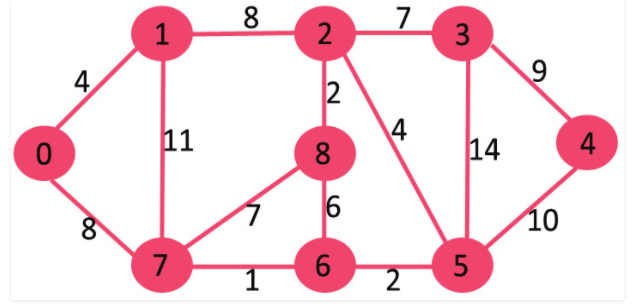
\includegraphics[scale=0.7]{gfx/fig31.png}\\\\
\textit{Solution:}\\\\
Assign cost value of $\infty$ for all nodes which are not directly connected to node "0", and compute the distance for the nodes "1" and "7".\\\\
\begin{tabular}{c | c| c| c| c| c| c| c| c}
	from/To & 1 & 2 & 3 & 4 & 5 & 6 & 7 & 8 \\
	\hline
	0 & 4* & $\infty$ & $\infty$& $\infty$& $\infty$& $\infty$ & 8 & $\infty$\\
\end{tabular}\\\\
Since $ 4 < 8 $, we will assign node "7" as our next vertex, then:\\\\
\begin{tabular}{c | c| c| c| c| c| c| c| c}
	from/To & 1 & 2 & 3 & 4 & 5 & 6 & 7 & 8 \\
	\hline
	0 & 4* & $\infty$ & $\infty$& $\infty$& $\infty$& $\infty$ & 8 & $\infty$\\
	1 & - & 12 & $\infty$& $\infty$& $\infty$& $\infty$ & 8* ($\because 8 < 15$) & $\infty$\\
\end{tabular}\\\\
In the above step, we assigned the value 8 for node "7", because $ 8 < 15 $(computed value from node "1"). Also, in this step, since $ 8 < 12 $, we will assign node "7" as our next vertex, then:\\\\
\begin{tabular}{c | c| c| c| c| c| c| c| c}
	from/To & 1 & 2 & 3 & 4 & 5 & 6 & 7 & 8 \\
	\hline
	0 & 4* & $\infty$ & $\infty$& $\infty$& $\infty$& $\infty$ & 8 & $\infty$\\
	1 & - & 12 & $\infty$& $\infty$& $\infty$& $\infty$ & 8* & $\infty$\\
	7 & - & 12 & $\infty$& $\infty$& $\infty$& 9* & - & 15\\
\end{tabular}\\\\
In the above step, node "7" is not directly connected to node "2" and the node is not solved yet, so the value remains as it is. Since, $ 9 < 12 < 15 $, we assign node "6" as our next vertex, then:\\\\
\begin{tabular}{c | c| c| c| c| c| c| c| c}
	from/To & 1 & 2 & 3 & 4 & 5 & 6 & 7 & 8 \\
	\hline
	0 & 4* & $\infty$ & $\infty$& $\infty$& $\infty$& $\infty$ & 8 & $\infty$\\
	1 & - & 12 & $\infty$& $\infty$& $\infty$& $\infty$ & 8* & $\infty$\\
	7 & - & 12 & $\infty$& $\infty$& $\infty$& 9* & - & 15\\
	6 & - & 12 & $\infty$& $\infty$& 11* & - & - & 15 \\
\end{tabular}\\\\
In the above step, the computed value for node "8" from node "6" was 15, since the value didn't change we set the value as it is, that is, 15. Also, $ 11 < 12 < 15 $, so we assign node "5" as our next vertex, then:\\\\
\begin{tabular}{c | c| c| c| c| c| c| c| c}
	from/To & 1 & 2 & 3 & 4 & 5 & 6 & 7 & 8 \\
	\hline
	0 & 4* & $\infty$ & $\infty$& $\infty$& $\infty$& $\infty$ & 8 & $\infty$\\
	1 & - & 12 & $\infty$& $\infty$& $\infty$& $\infty$ & 8* & $\infty$\\
	7 & - & 12 & $\infty$& $\infty$& $\infty$& 9* & - & 15\\
	6 & - & 12 & $\infty$& $\infty$& 11* & - & - & 15 \\
	5 & - & 12* ($\because 12 < 15$) & 25 & 21 & - & - & - & 15 \\
\end{tabular}\\\\
In the above step, the computed value for node "2" from node "5" was 15, and since $ 12 < 15 $, we retain the earlier value, that is, 12. Also, $ 12 < 15 < 21 < 25 $, we assign node "2" as our next vertex, then:\\\\
\begin{tabular}{c | c| c| c| c| c| c| c| c}
	from/To & 1 & 2 & 3 & 4 & 5 & 6 & 7 & 8 \\
	\hline
	0 & 4* & $\infty$ & $\infty$& $\infty$& $\infty$& $\infty$ & 8 & $\infty$\\
	1 & - & 12 & $\infty$& $\infty$& $\infty$& $\infty$ & 8* & $\infty$\\
	7 & - & 12 & $\infty$& $\infty$& $\infty$& 9* & - & 15\\
	6 & - & 12 & $\infty$& $\infty$& 11* & - & - & 15 \\
	5 & - & 12* & 25 & 21 & - & - & - & 15 \\
	2 & - & - & 19 ($\because 19 < 25$)& 21 & - & - & - & 14* ($\because 14 < 15$)\\
\end{tabular}\\\\
in the above step, since $ 14 < 19 < 21 $, we assign node "8" as our next vertex, then:\\\\
\begin{tabular}{c | c| c| c| c| c| c| c| c}
	from/To & 1 & 2 & 3 & 4 & 5 & 6 & 7 & 8 \\
	\hline
	0 & 4* & $\infty$ & $\infty$& $\infty$& $\infty$& $\infty$ & 8 & $\infty$\\
	1 & - & 12 & $\infty$& $\infty$& $\infty$& $\infty$ & 8* & $\infty$\\
	7 & - & 12 & $\infty$& $\infty$& $\infty$& 9* & - & 15\\
	6 & - & 12 & $\infty$& $\infty$& 11* & - & - & 15 \\
	5 & - & 12* & 25 & 21 & - & - & - & 15 \\
	2 & - & - & 19 & 21 & - & - & - & 14*\\
	8 & - & - & 19* & 21 & - & - & - & -\\
\end{tabular}\\\\
In the above step, node "8" had no direct connection with either of the unsolved nodes, "3" and "4", so we resolve to assign node "3" as our next vertex as $ 19 < 21 $, then:\\\\
\begin{tabular}{c | c| c| c| c| c| c| c| c}
	from/To & 1 & 2 & 3 & 4 & 5 & 6 & 7 & 8 \\
	\hline
	0 & 4* & $\infty$ & $\infty$& $\infty$& $\infty$& $\infty$ & 8 & $\infty$\\
	1 & - & 12 & $\infty$& $\infty$& $\infty$& $\infty$ & 8* & $\infty$\\
	7 & - & 12 & $\infty$& $\infty$& $\infty$& 9* & - & 15\\
	6 & - & 12 & $\infty$& $\infty$& 11* & - & - & 15 \\
	5 & - & 12* & 25 & 21 & - & - & - & 15 \\
	2 & - & - & 19 & 21 & - & - & - & 14*\\
	8 & - & - & 19* & 21 & - & - & - & -\\
	3 & - & - & - & 21* ($\because 21 < 28$) & - & - & - & -\\
\end{tabular}\\\\
Hence, the shortest distance from node "0" to all other nodes are given below:\\\\
\begin{tabular}{c | c}
	\textbf{node} & \textbf{shortest distance from node "0"/source}\\
	\hline
	1 & 4\\
	2 & 12\\
	3 & 19\\
	4 & 21\\
	5 & 11\\
	6 & 9\\
	7 & 8\\
	8 & 14
\end{tabular}\\\\
Hence the shortest route to reach node "4" from node "0" is 0-7-6-5-4.
%
\section{Review Problems}
\begin{enumerate}
	\item Define the term public transportation. Briefly describe the different types of transit modes in public transportation.
	\item List out the factors which are good and bad for transit.
	\item Derive the expression for headway determination by "Square Root Formula".
	\item Derive the expression for Transit Line Capacity, and use the expression to determine the average transit line utilization($\alpha$).
	\item Let us assume that transit line parameters are respectively equal: $ c = 120\$ $ per hour, $\nu$ = 12\$ per passenger hour, $r$ = 1400 passengers per hour, and $T$ = 120 min = 2hr. Calculate the optimal headway by using the “square root formula.”
	\item Derive an expression for the the average number of times a transit
	unit stops, $ E(s) $, and use the relation to illustrate the relationship between stopping policy and demand.
	\item Describe the properties of a good route set.
	\item Discuss the properties of a good schedule.
	\item The transit operator monitored during 10 days period the daily number of passengers that departed from the station \#5. The following 10 values were recorded: 1160, 1245, 1440, 1280, 1180, 1380, 1220, 1358, 1178 and 1382. The maximum number of passengers per car is equal to 100. The transit operator would like to achieve the load factor that is equal to 0.75. Calculate the average value of the maximum daily passenger volumes. Determine the service frequency f that should be offered in order to satisfy maximum passenger volume and the desired vehicle occupancy.
	\item The public transit line length equals 12 km in one direction. The average bus speed on a city heavy traffic equals 25 km/h. The total of 14 buses is assigned to the line. The capacity of every vehicle equals 60. Calculate the line capacity, frequency, and headway.
	\item Calculate the shortest path from node "A" to all other nodes, and also determine the shortest route from node "A" to node "G".
	\begin{center}
		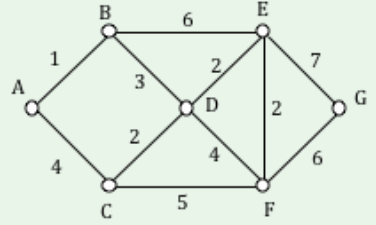
\includegraphics{gfx/fig32.png}
	\end{center}
	\item The number of boarding passengers, number of alighting passengers and the number of passengers in the vehicle are given in the following table:\\\\
	\begin{tabular}{c | c | c}
		\textbf{Bus stop} & \textbf{\# of boarding passengers} & \textbf{\# of alighting passengers} \\
		\hline
		Terminal A & 9 & 0\\
		1 & 10 & 6\\
		2 & 14 & 4\\
		3 & 9 & 11\\
		4 & 7 & 17\\
		5 & 0 & 7\\
		Terminal B & 0 & 4\\
		\hline
	\end{tabular}\\\\
	Graphically illustrate the number of boarding passengers, number of alighting passengers and the number of passengers in the vehicle for all line sections. Also, graphically show the passenger load profile and identify the Maximum Load Section (MLS).
	\item A public transit operator wants to provide service frequency between 6:00 and 7:00 that is equal to 4. Between 7:00 am and 8:00 am the operator wants to offer service frequency equals to 6. The operator provides service frequency that is equal to 8 in the time interval between 8:00 am and 9:00 am. Generate vehicles timetable that will provide constant vehicle headways within time interval from 6:00 am to 9:00 am. Show the solution graphically.
\end{enumerate}